\documentclass[times, utf8, seminar]{fit}

%\batchmode
%\usepackage{booktabs}
\usepackage{listings}
\usepackage{longtable}
\usepackage{xcolor}
\usepackage{float}
\usepackage{enumitem}
\usepackage{hyperref}
\usepackage{enumerate}
\usepackage{graphicx}
\usepackage{etoolbox}
\usepackage{datetime}
\usepackage{needspace}
\usepackage{titlesec}
%\titleformat{\chapter}[display]{\normalfont\huge\bfseries}{\chaptertitlename\ \thechapter}{20pt}{\Huge}

\begin{document}
\widowpenalty=300
\clubpenalty=300


% this alters "before" spacing (the second length argument) to 0
%\titlespacing*{\chapter}{0pt}{0pt}{40pt}

% this changes "before" spacing back to its default of 50pt
%\titlespacing*{\chapter}{0pt}{50pt}{40pt}}

%\titlespacing*{\chapter}{0pt}{-50pt}{18pt}
%\titleformat{\chapter}[display]{\normalfont\huge\bfseries}{\chaptertitlename\ \thechapter}{20pt}{\Huge}

\title{OSS e-commerce rješenje sa sistemom preporuke}

\author{Ernad Husremović}
\brindex{DL 2792}
\verzija {0.9.1}

\mentor{mr. Haris Balta}

\maketitle

\tableofcontents

%\listoftables
%\listoffigures
\newpage

% abstract begin
%\begin{abstract}
%
%To be done 
%
%\keywords{open source software, OSS, Bosna i Hercegovina}
%\end{abstract}

% abstract end

\chapter{Uvod}
\vspace*{-0.7cm}

Cilj ovog seminarskog rada je implementirati webshop rješenje čije su komponente isključivo open source (nadalje OSS) software-a 

Firma "bring.out", implementator sistema je bosanski OSS IT provajder.

Kompletan portfolio firme je baziran na OSS-u, tako da i ovo rješenje treba zadovoljiti kriterije otvorenosti izvornog koda.

\chapter{Analiza dostupnih OSS komponenti za gradnju rješenja}
\vspace*{-0.7cm}

\section{Sistemi preporuke}

Najpoznatiji OSS sistemi preporuke su:

\begin{itemize}
  \item easyrec\footnote{\url{http://easyrec.org/}}
  \item Apache mahout\footnote{\url{http://mahout.apache.org/}}
  \item Lenskit recommender framework\footnote{\url{http://lenskit.grouplens.org/}}
\end{itemize}

\emph{Apache mahout} je projekat koji ima reputaciju najkopletnijeg i najkompleksnijeg "recommendation engine"-a 

Postoji odična integracija sa drugim projektom popularnim "Apache fondacije" - hadoop-om\footnote{\url{http://hadoop.apache.org}} koji se koristi u za distribuiranu obradu "big data"\footnote{velike količine podataka, najčešće korišteno u  rješenjima "data-mining" sistema}.

Sva tri pomenuta rješenja su implementirana u programskom jeziku Java.

\emph{Lenskit} je najmlađi projekat, ali ima veoma aktivnu zajednicu korisnika i programera (eng. "community").

\emph{Easyrec} je započeo kao komercijalni projekat austrijske firme "Studio Smart Agent Technologies". Naknadno je objavljen kao OSS pod GPLv3 licencom. 
Dobio je više nagrada za inovaciju na području web-a i multimedije\footnote{\url{http://en.wikipedia.org/wiki/Easyrec}}. 
Easyrec je java aplikacija koja sa webshop rješenjima komunicira putem web servisa (REST ili SOAP), tako da je moguća integracija sa bilo kojim third-party sistemom.
Sadrži kvalitetan web administrativni interfejs izdvaja od konkurentskih rješenja.

\begin{figure}[H]
\centering
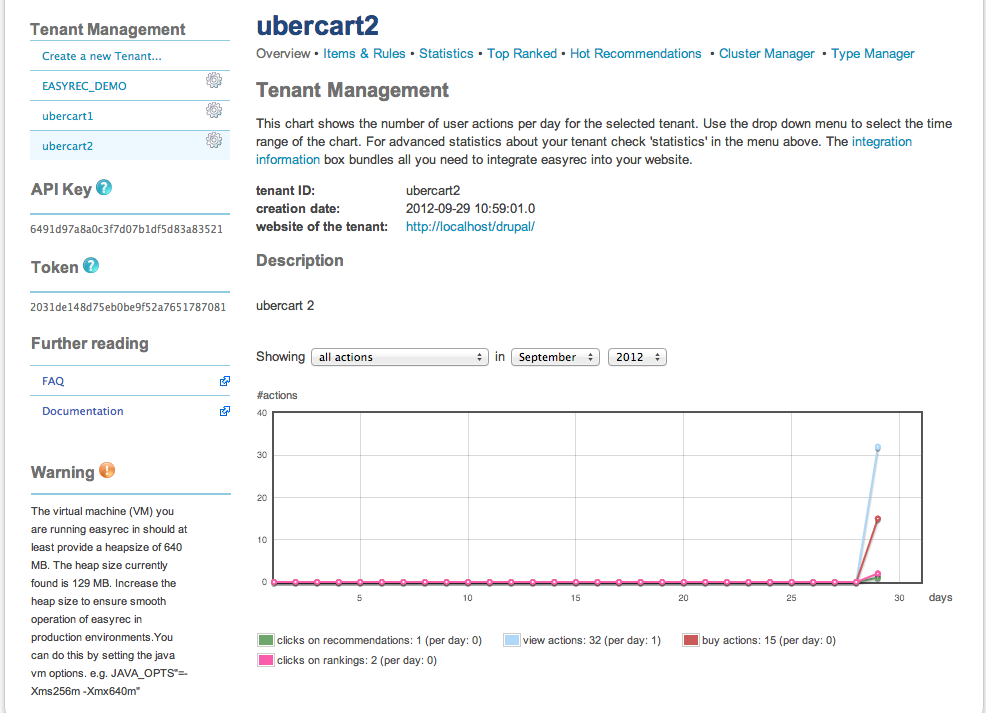
\includegraphics[width=10cm]{img/easyrec_1_tenant.png}
\caption{Easyrec web interfejs}
\end{figure}



\section{Web shop rješenje}

Postoji niz OSS rješenja. Međutim, sa stanovišta proširivosti, "drupal"{\footnote{\url{http://www.drupal.org}} bazirana rješenja su najpopularnija.

\subsection{Drupal web content framework}

Drupal je "web content framework" napisan u programskom jeziku PHP. 

Često se navodi i da je drupal "CMS"{\footnote{CMS - Content Management System}} software, međutim framework je definitivno bolji opis drupal-a.

Drupal je razvojna platforma za različite web sadržaje.

\begin{figure}[H]
\centering
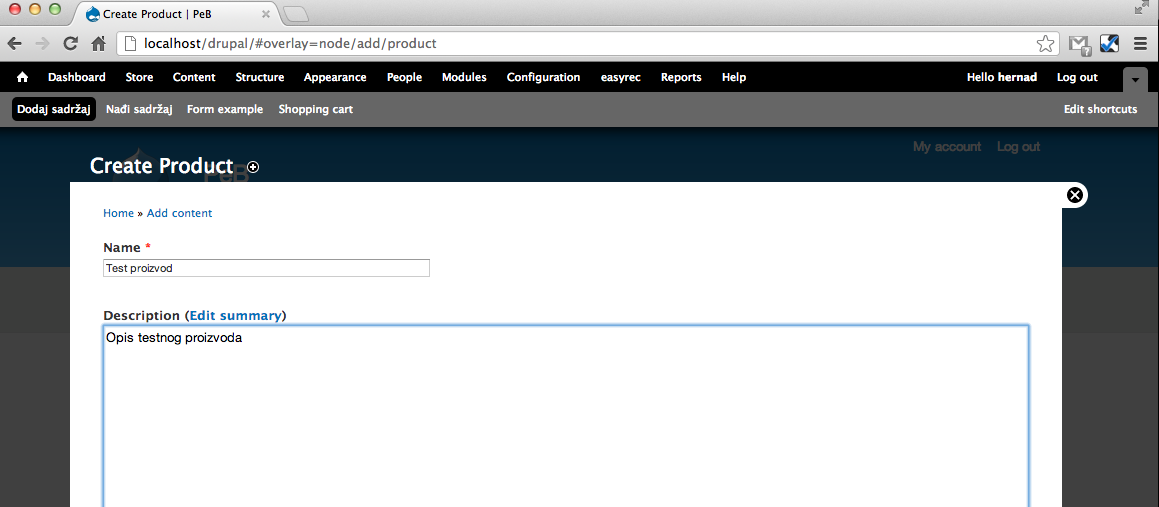
\includegraphics[width=10cm]{img/drupal_add_content.png}\hfill
\caption{Drupal web interfejs dodavanje sadržaja (content)}
\end{figure}

\begin{figure}[H]
\centering
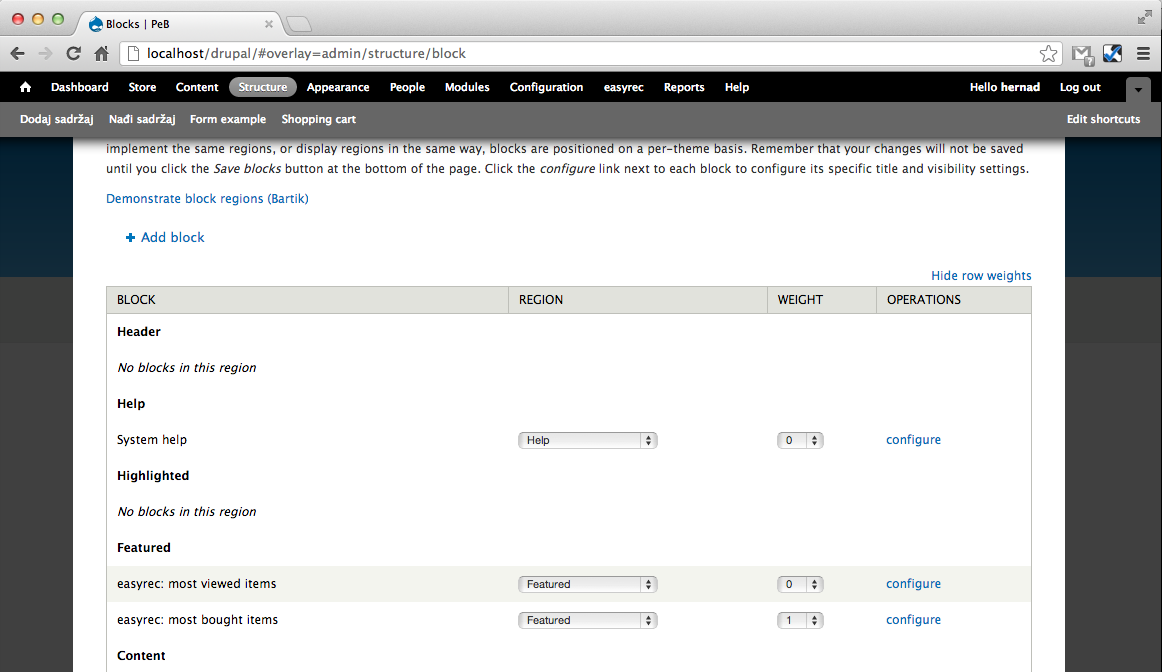
\includegraphics[width=10cm]{img/drupal_block_structure.png}\hfill
\caption{Drupal web interfejs - podešenje strukture prikaza (blocks)}
\end{figure}


%\begin{center}
%\emph{\large{Freedom to create, distribute, and use open source software (OSS).}}
%\end{center}

\subsection{OSS E-commerce rješenja}

Na tržištu postoji više OSS aktivnih drupal e-commerce projekata:

\begin{itemize}
\ubercart  
\item drupal commerce\footnote{\url{http://www.drupalcommerce.org}} 
\item ubercart\footnote{\url{http://www.ubercart.org}}
\end{itemize}

"Drupal comerce" je relativno mlad projekat, ali je vrlo brzo stekao vidljivost na tražištu OSS e-commerce rješenja.

Započeli su ga bivši developer "ubercart"-a, koji je opet prvo "ozbiljno" OSS e-commerce rješenje.

Web stranice prokejkta ukazuju da se radi o ozbiljnom projektu sa jakom finansijskom podrškom:

\begin{figure}[H]
\centering
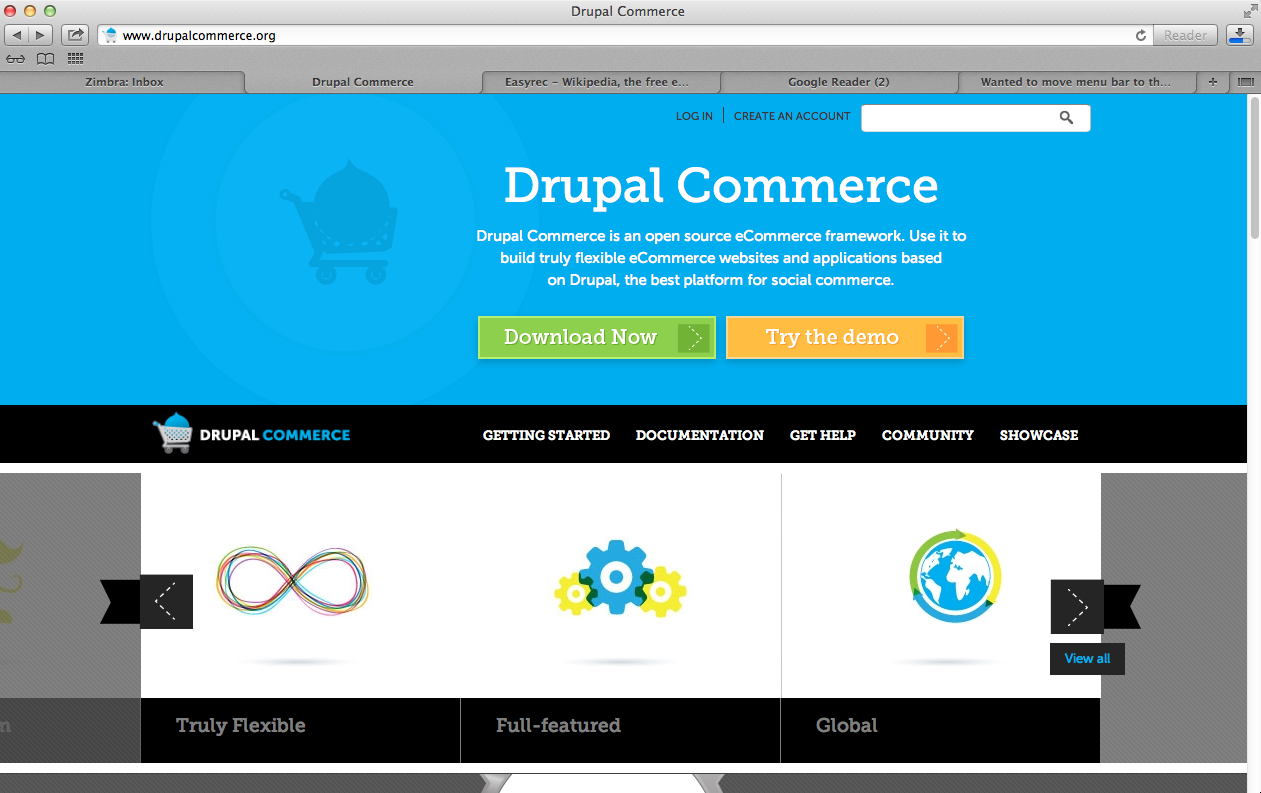
\includegraphics[width=4.5cm]{img/drupalcommerce_web.png}\hfill
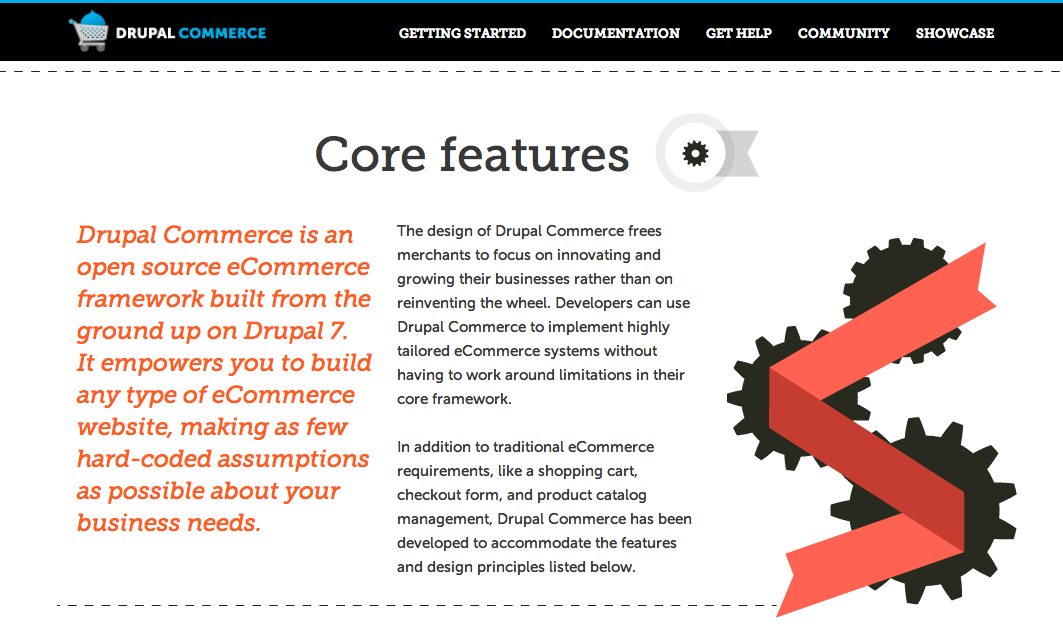
\includegraphics[width=4.5cm]{img/drupalcommerce_web_2.png}\hfill
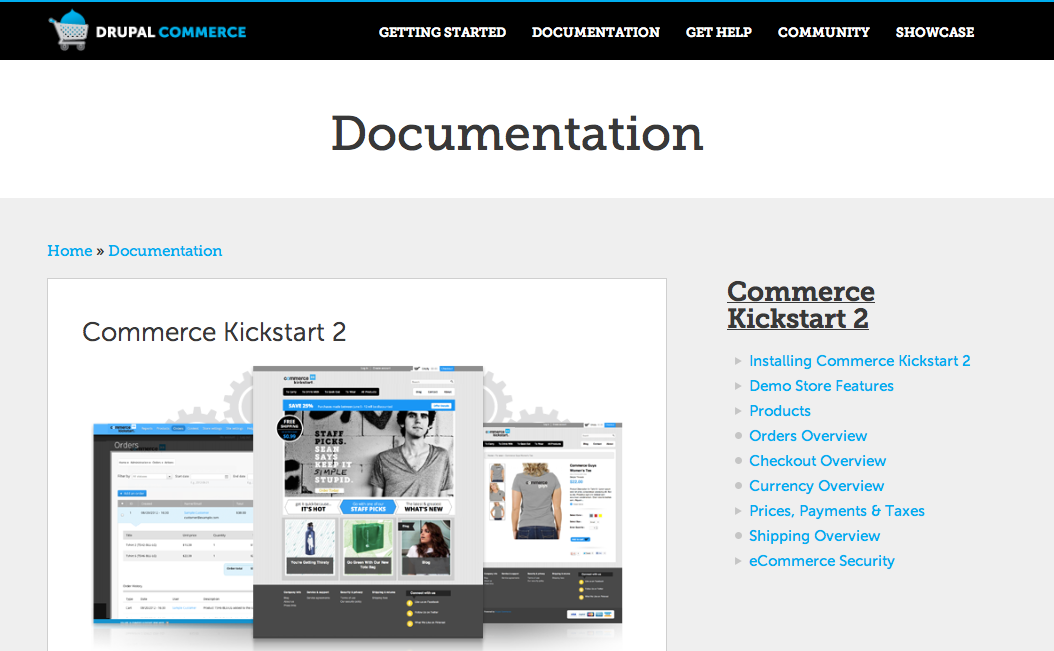
\includegraphics[width=4.5cm]{img/drupalcommerce_web_3.png} 
\caption{Drupal commerce web site}
\end{figure}

Filozofija razvoja drupal commerce-a je slična razvoju samog drupala. Drupalcommerce je core sistem za nove e-commerce distribucije koje su bazirane na njemu.
Source code je GPLv2 licenciran kao i sam drupal.

\emph{Ubercart} je svojevrsni "veteran" drupal baziranih e-commerce rješenja. Ubercart v2.x (baziran na drupal 6.x) je vrlo zastupljen e-commerce sistem.

\subsection{Integracijska komponenta (e-commerce <-> sistem preporuke)}

Posljednja komponenta u konstrukciji zadanog sistema je integracijska komponenta e-commerce <-> recommender.

Ubercart ima riješenu integraciju sa easyrec-om kao poseban drupal projekat{\footnote{\url{http://drupal.org/project/easyrec\_for\_ubercart}} 

\section{Odabir komponenti}

Easyrec se svojom jednostavnošću i fleksibilnošću odmah nametnuo kao dobar izbor za komponentu koja će biti sistem preporuke. 
Kako za njega postoji i integracijska komponenta sa ubercart-om konačan izbor sistema je:
\begin{enumerate}
  \item drupal 7.x
  \item ubercart 3.x
  \item easycart 0.97
  \item easyrec\_for\_ubercart
\end{enumerate}

%\begin{quotation}
%\emph{In 2009, more than four out of 10 software programs installed on personal computers around the world were stolen, with a commercial value of more than \$51 billion. Unauthorized software can manifest in otherwise legal businesses that buy too few software licenses, or cover criminal enterprises that sell counterfeit copies of software programs at cut-rate prices, online or offline.}

%\emph{However, the impact of software piracy goes beyond revenues lost to the software industry, starving local software distributors and service providers of spending that creates jobs and generates much-needed tax revenues for governments around the world.}\citep{bsapiracyimpact}
%\end{quotation}\\

%\chapter{OSS in Bosnia and Herzegovina}

\chapter{Instalacija}
\vspace*{-0.7cm}
\setlength{\parindent}{0cm}
%\setlength{\parindent}{default}

\section{Bazno okruženje}

\subsection{XAMPP PHP, Mysql database server}
Drupal instaliramo unutar  XAMPP stack-a{\footnote{\url http://www.apachefriends.org/en/xampp.html} za Mac OS X 1.7.3 (MySQL 5.1.x, PHP 5.3.x)

\lstset{
  language=bash,
  backgroundcolor=\color{gray!25},
  basicstyle=\ttfamily \footnotesize,
  breaklines=true,
  prebreak=\raisebox{0ex}[0ex][0ex] \hookleftarrow,
  columns=fullflexible
}

%\lstset{
%}
%\lstset{postbreak=\raisebox{0ex}[0ex][0ex] \rcurvearrowse\space}
%\lstset{breaklines=true, breakatwhitespace=true}
%\lstset{numbers=left, numberstyle=\scriptsize}

Apache web server web root:
\begin{lstlisting}
/Applications/XAMPP/htdocs
\end{lstlisting}

\subsection{Easyrec web aplikacija}

Easyrec je stanardna J2EE\footnote{java enterprise edition} web aplikacija (WAR), tako da za njegovu instalaciju trebamo J2EE aplikacijski server. 

Preporučeni server je tomcat. Instaliramo tomcat, kopiramo easyrec-web.war (ver. 0.97)\footnote{download sa sourceforge repozitorija \url{http://sourceforge.net/projects/easyrec/files/}} u deployment direktorij tomcat servera i na kraju pokrećemo server:

\begin{lstlisting}

1) ~/FIT/PeB/apache-tomcat-7.0.30$ cp ~/Downloads/easy-rec.war webapps/

2) ~/FIT/PeB/apache-tomcat-7.0.30/bin\$ ./catalina.sh start

> Using CATALINA_BASE:   /Users/hernad/FIT/PeB/apache-tomcat-7.0.30
> Using CATALINA_HOME:   /Users/hernad/FIT/PeB/apache-tomcat-7.0.30
> Using CATALINA_TMPDIR: /Users/hernad/FIT/PeB/apache-tomcat-7.0.30/temp
> Using JRE_HOME:        /System/Library/Frameworks/JavaVM.framework/Versions/CurrentJDK/Home
> Using CLASSPATH:       /Users/hernad/FIT/PeB/apache-tomcat-7.0.30/bin/bootstrap.jar:/Users/hernad/FIT/PeB/apache-tomcat-7.0.30/bin/tomcat-juli.jar
\end{lstlisting}

Pokrećemo u browseru 

\begin{lstlisting}
http://localhost:8080/easyrec-web
\end{lstlisting}

prolazimo kroz jednostavni install proces koji u easyrec bazu\footnote{koju ranije trebamo kreirati, vidi donji korak "Kreiranje easyrec baze"} 

Na kraju dobijamo dolazimo na login našeg sistema preporuke:

\subsection{Kreiranje drupal i easyrec baza}

\begin{lstlisting}
/Applications/XAMPP/xamppfiles$ bin/mysql -u root
mysql> create database ubercart3;

> Query OK, 1 row affected (0.07 sec)

mysql> create database easyrec;

mysql> quit

\end{lstlisting}

\subsection{Drupal}

Drupal core 7.1.15 sa svim potrebni podmodulima nalazi se na hernad github repozitoriju. 

Izvršimo kloniranje repozitorija i njegovih podmodula:

\begin{lstlisting}
1) /Applications/XAMPP/htdocs$ git clone git@github.com:hernad/drupal.git

>  Cloning into 'drupal'...

/Applications/XAMPP/htdocs$ cd drupal

2) /Applications/XAMPP/htdocs/drupal$ git submodule init 

> Submodule 'sites/all/modules/easyrec_for_ubercart' (git@github.com:hernad/easyrec_for_ubercart.git) registered for path 'sites/all/modules/easyrec_for_ubercart'
> Submodule 'sites/all/modules/jcarousel' (git@github.com:hernad/jcarousel.git) registered for path 'sites/all/modules/jcarousel'
> Submodule 'sites/all/modules/ubercart' (git@github.com:hernad/ubercart.git) registered for path 'sites/all/modules/ubercart'

3) /Applications/XAMPP/htdocs/drupal$ git submodule update

> Cloning into 'sites/all/modules/easyrec_for_ubercart'...
> ...
> Submodule path 'sites/all/modules/easyrec_for_ubercart': checked out '26a96e622be0acee012c4cff85b3e8e4f87cd5e5'
> Cloning into 'sites/all/modules/jcarousel'...
> ....
> Submodule path 'sites/all/modules/jcarousel': checked out 'ef51d00eae77e354c771cf595621971f5f250ac2'
> Cloning into 'sites/all/modules/ubercart'...
> ...
> Submodule path 'sites/all/modules/ubercart': checked out 'e5a4154d8a9fdf6483fabd7e851798f3c88fd623'
\end{lstlisting}

Podešenje drupal config fajlova:

\begin{lstlisting}
/Applications/XAMPP/htdocs/drupal/sites$ cp example.sites.php sites.php
/Applications/XAMPP/htdocs/drupal/sites$ chmod a+w sites.php
/Applications/XAMPP/htdocs/drupal/sites$ mkdir -p default/files
/Applications/XAMPP/htdocs/drupal/sites$ chmod a+w default/files
/Applications/XAMPP/htdocs/drupal/sites$ cd default
/Applications/XAMPP/htdocs/drupal/sites/default$ cp default.settings.php  settings.php
/Applications/XAMPP/htdocs/drupal/sites/default$ chmod a+w settings.php
/Applications/XAMPP/htdocs/drupal/sites/default$ cd ..
\end{lstlisting}

\begin{figure}[H]
\centering
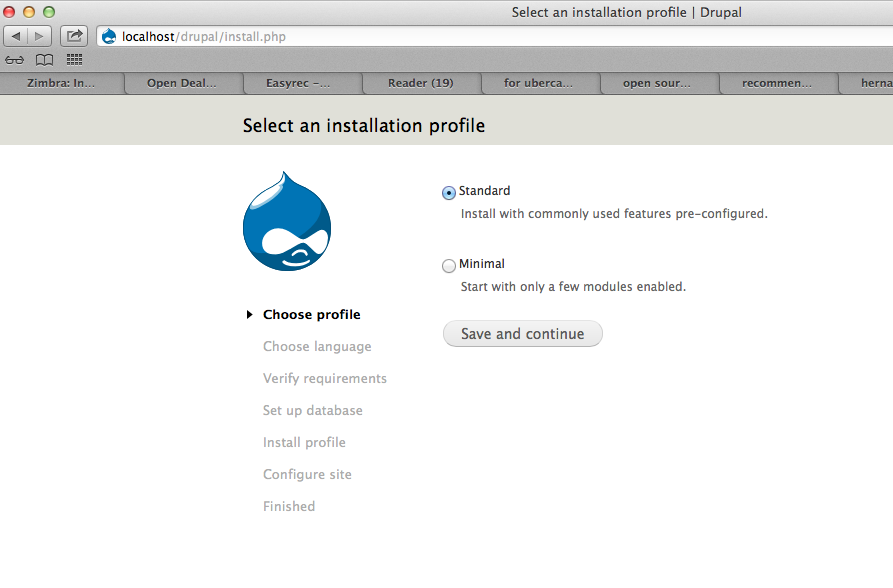
\includegraphics[width=10cm]{img/drupal_install_1.png}
\caption{Drupal install step 1}
\end{figure}

\begin{figure}[H]
\centering
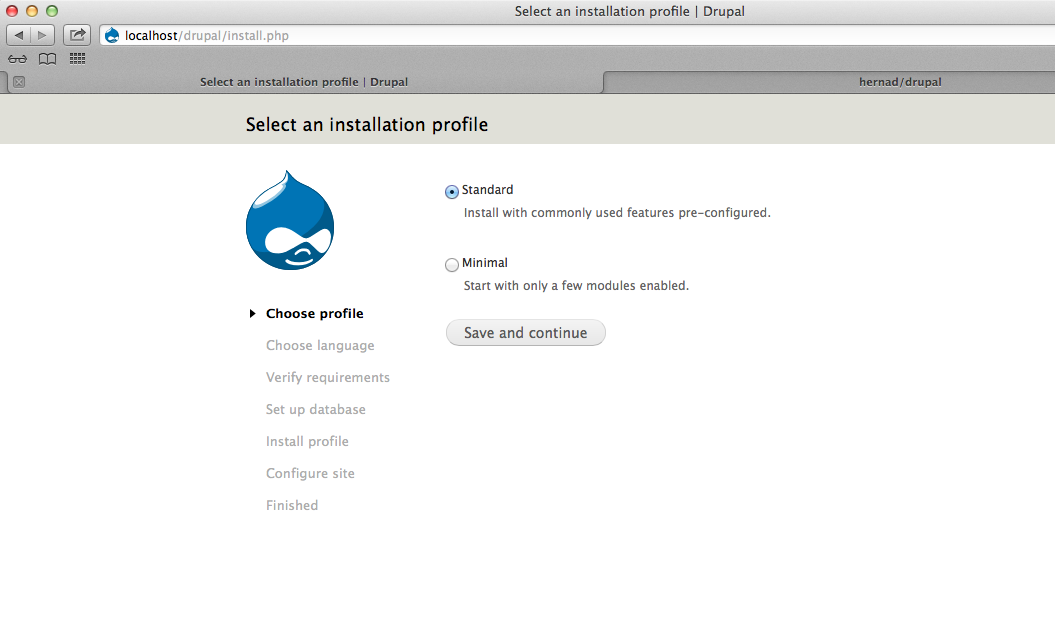
\includegraphics[width=10cm]{img/drupal_install_2.png}
\caption{Drupal install step 2}
\end{figure}

\begin{figure}[H]
\centering
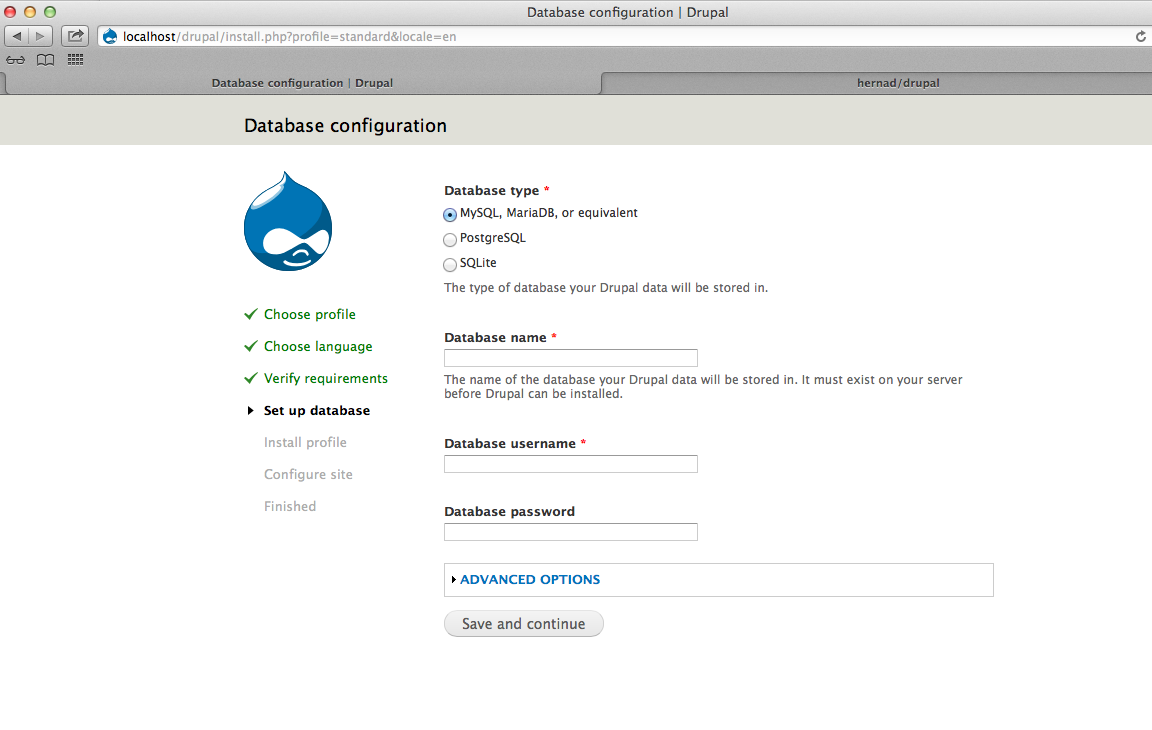
\includegraphics[width=10cm]{img/drupal_install_3.png}
\caption{Drupal install step 3}
\end{figure}

\begin{figure}[H]
\centering
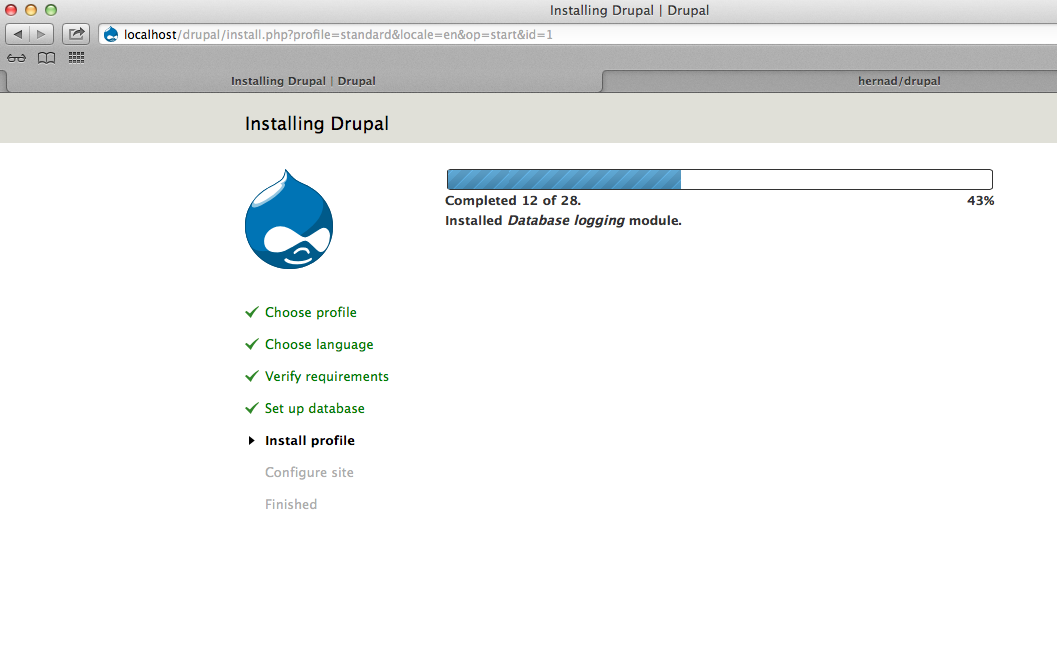
\includegraphics[width=10cm]{img/drupal_install_4.png}
\caption{Drupal install step 4}
\end{figure}

\begin{figure}[H]
\centering
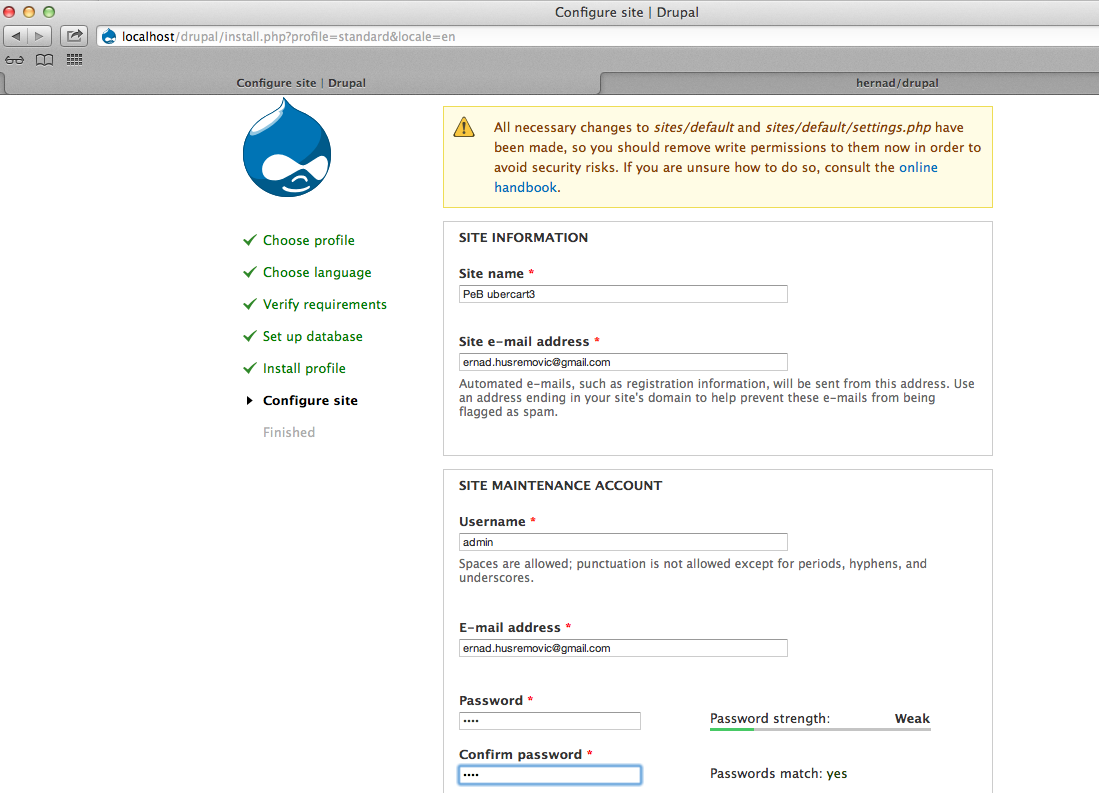
\includegraphics[width=9cm]{img/drupal_install_5.png}
\caption{Drupal install step 5}
\end{figure}

\begin{figure}[H]
\centering
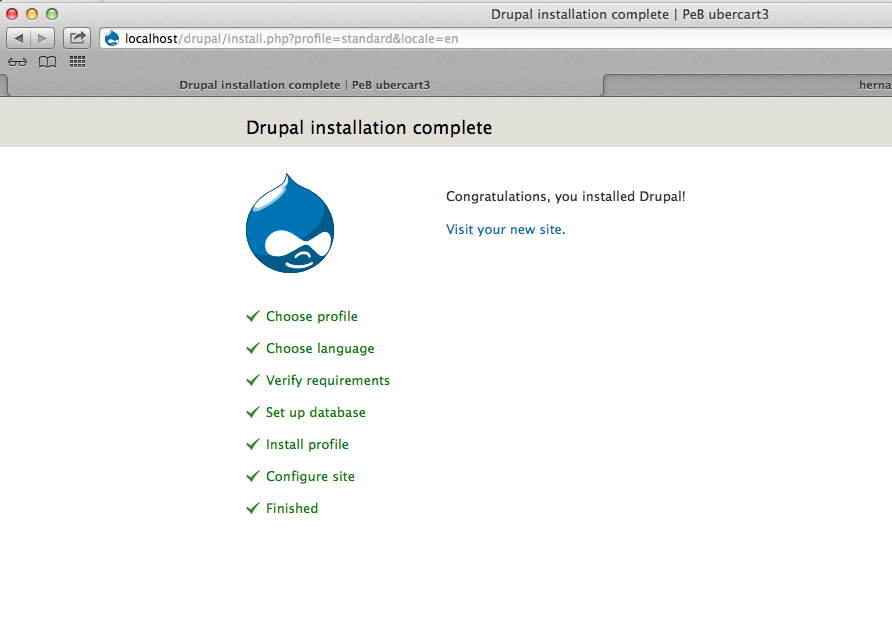
\includegraphics[width=9cm]{img/drupal_install_6.png}
\caption{Drupal install step 6}
\end{figure}


\begin{figure}[H]
\centering
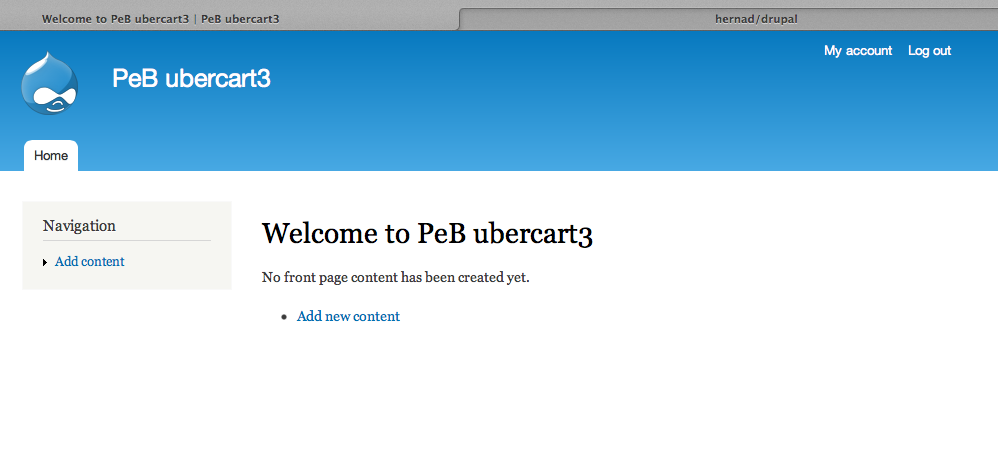
\includegraphics[width=12cm]{img/drupal_welcome.png}
\caption{Drupal install - napokon "welcome" :)}
\end{figure}

\subsection{Aktivacija drupal modula za ubercart i easyrec}

\begin{enumerate}
\item locale
\item chaost-tools
\item easyrec
\item rules
\item cart
\item store
\item order
\item product
\item views
\item views-ui
\end{enumerate}

\subsection{Podešenje drupal blokova za prikaz ubercart i easyrec elemenata}

Prikaz sadržaja na drupal stranicama se podešava unutar admin interfejsa.

Mi želimo na "featured" sekciju (vrh web stranice) staviti prikaz najviše kupovanih i najviše gledanih artikala u toku dana\footnote{Podešavamo dnevnu statistiku u testnom okruženju zato što se ona najprije ažurira}

\begin{figure}[H]
\centering
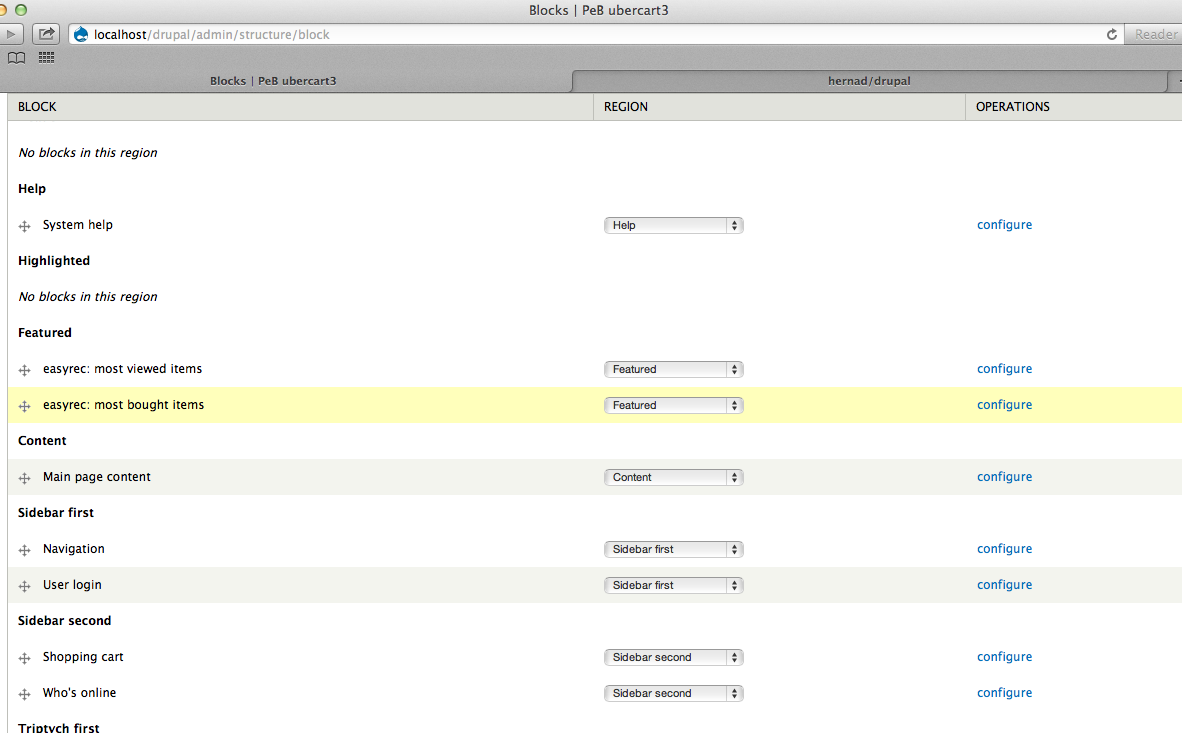
\includegraphics[width=12cm]{img/easyrec_ubercart_blocks_config_1.png}
\caption{Drupal block config}
\end{figure}

Ovako podešavamo prikaz najviše kupovanih artikala:

\begin{figure}[H]
\centering
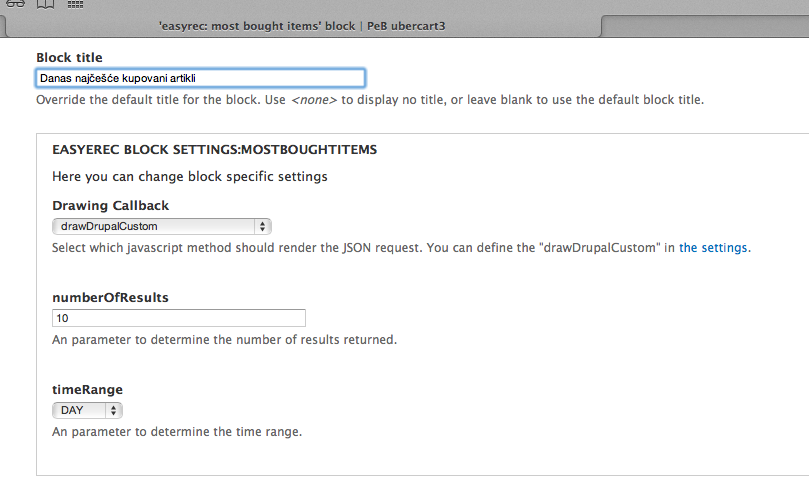
\includegraphics[width=12cm]{img/easyrec_ubercart_blocks_config_2.png}
\caption{Konfiguracija drupal blokova - prikaz sistema preporuke}
\end{figure}

Analogno se podešava i prikaz artikala koje su korisnici najviše pregledali.

\subsection{Podešenje komunikacije ubercart - easyrec server}

Dodajmo jedan "tenant" u easyrec\footnote{Inače tenant je u prevodu sa engleskog "stanar". U kontekstu easyrec-a, tenant je e-commerce aplikacije koju monitorišemo.}

\begin{figure}[H]
\centering
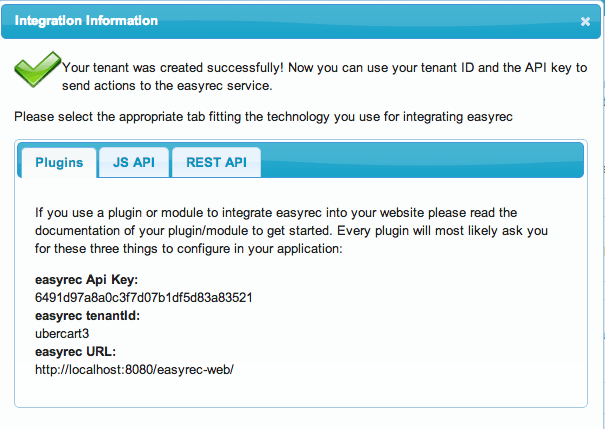
\includegraphics[width=12cm]{img/integ_easyrec.png}
\caption{Kreiranje novog tenanta ubercart3}
\end{figure}

Povezivanje drupala sa easyrec tenant-om "ubercart3":

\begin{figure}[H]
\centering
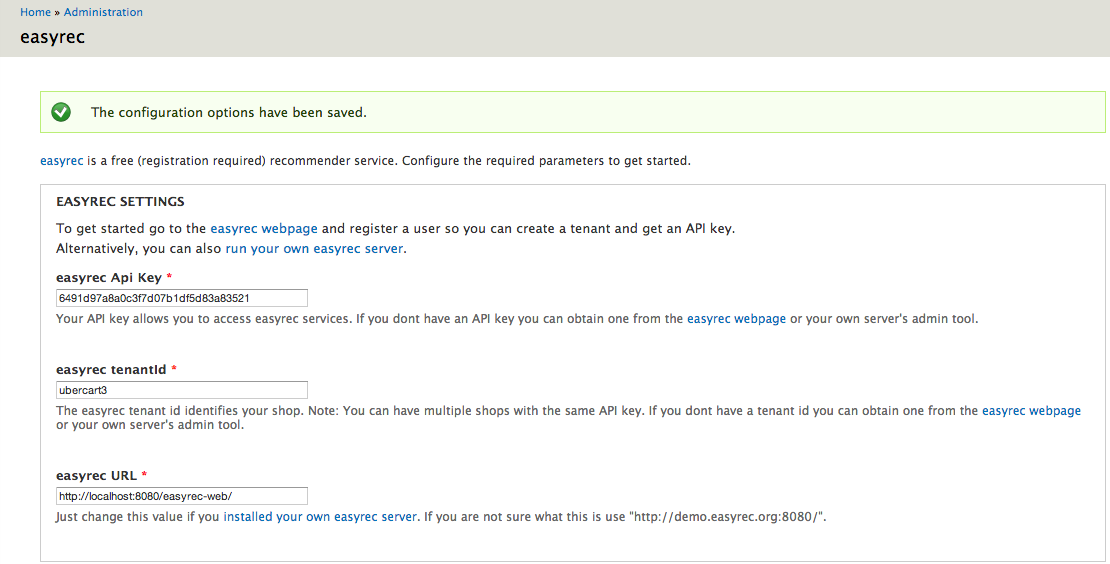
\includegraphics[width=12cm]{img/integ_drupal.png}
\caption{podešenje drupal easyrec modula}
\end{figure}

Nakon ovog podešenja, na easyrec web konzoli uočavamo da sistem bilježi "view" i "buy" akcije.

\chapter{Korištenje sistema}
\vspace*{-0.7cm}

\section{Definisanje artikla - proizvoda}

\begin{figure}[H]
\centering
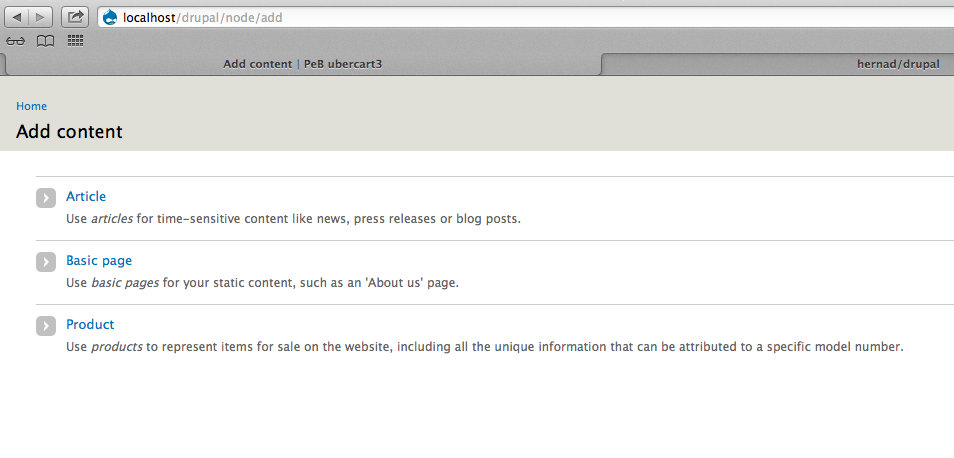
\includegraphics[width=10cm]{img/drupal_add_content_1.png}
\caption{Dodavanje novog proizvoda / 1}
\end{figure}


\begin{figure}[H]
\centering
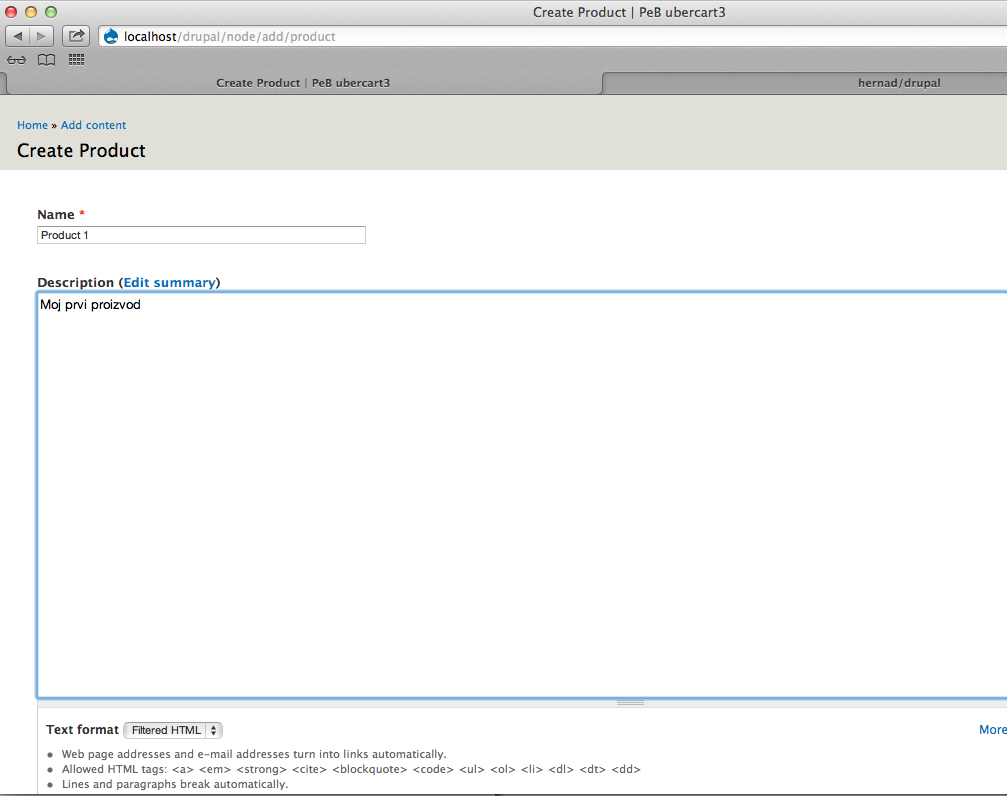
\includegraphics[width=10cm]{img/drupal_add_content_2.png}
\caption{Dodavanje novog proizvoda / 2}
\end{figure}

\begin{figure}[H]
\centering
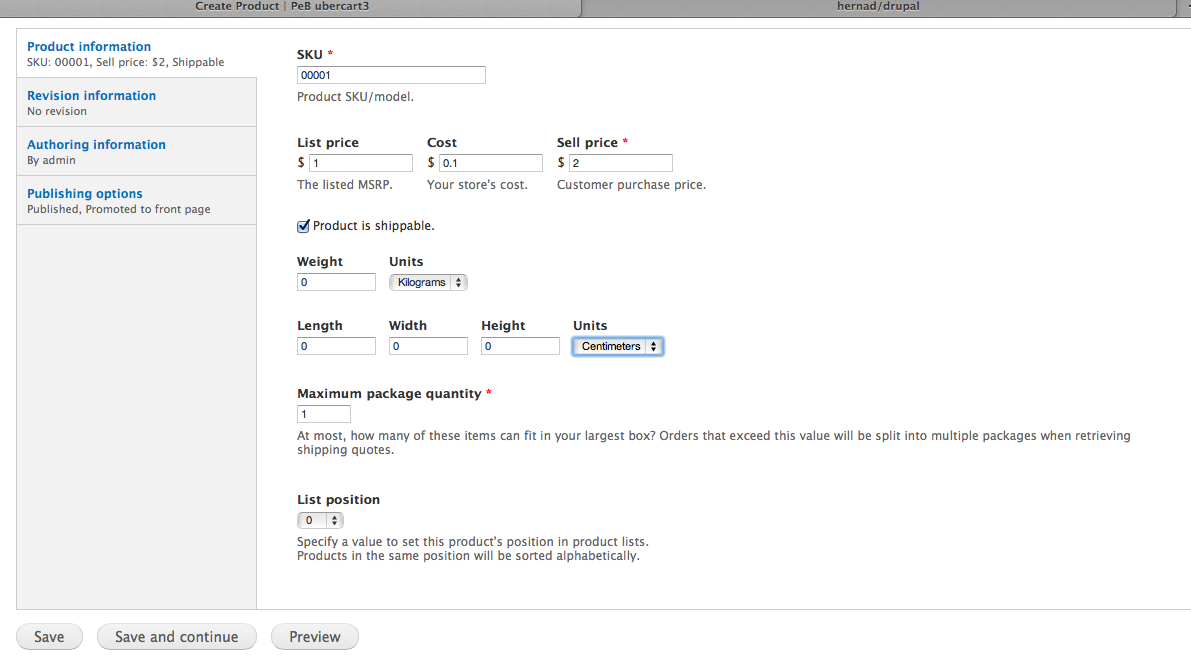
\includegraphics[width=10cm]{img/drupal_add_content_3.png}
\caption{Dodavanje novog proizvoda / 3}
\end{figure}

Na kraju, proizvod se prikazuje na naslovnoj stranici našeg web-shopa:

\begin{figure}[H]
\centering
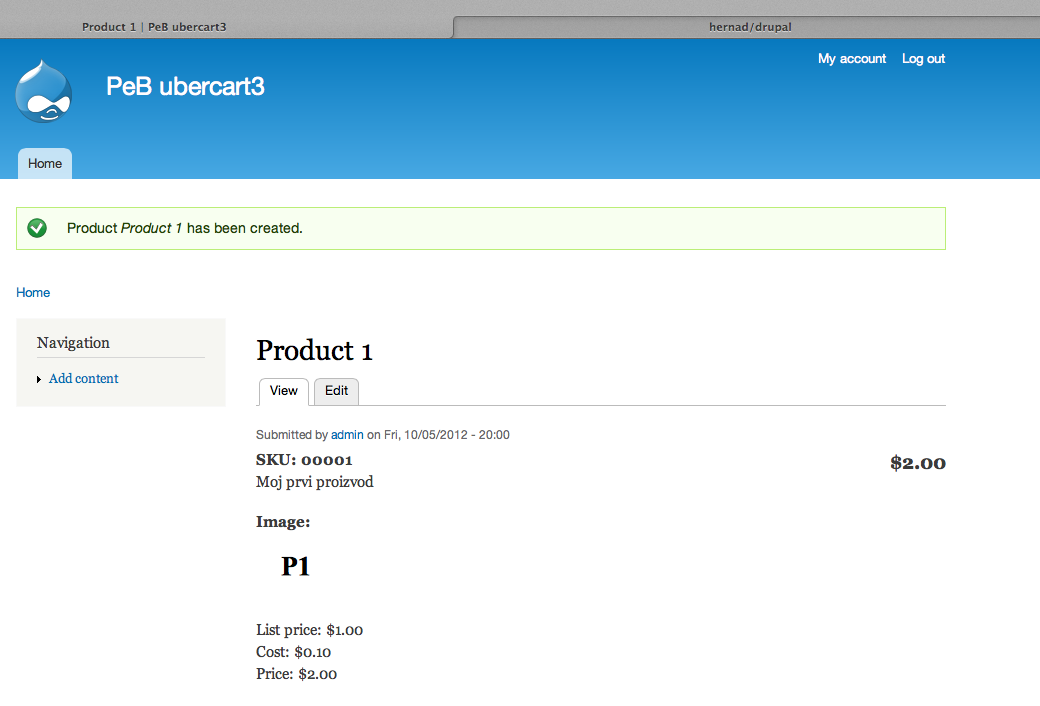
\includegraphics[width=10cm]{img/drupal_add_content_4.png}
\caption{Dodavanje novog proizvoda / 4}
\end{figure}

\section{Prodaja artikala}

Prodaja artikala unutar uberchart webshop rješenja je krajnje jednostavna. Klik na dugme proizvoda i korpa kupca se puni:

\begin{figure}[H]
\centering
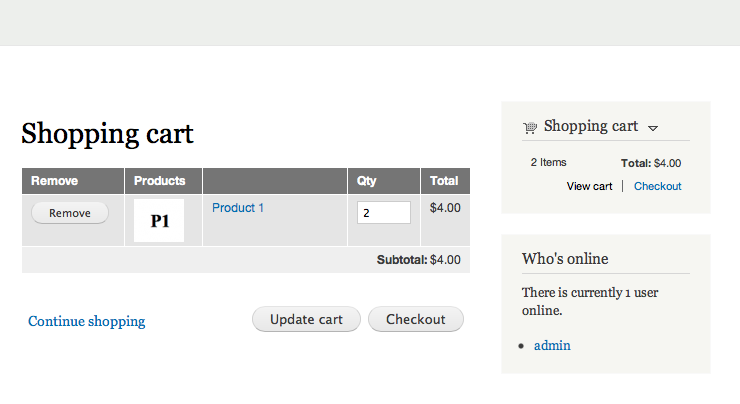
\includegraphics[width=10cm]{img/prodaja.png}
\caption{Potrošačka korpa "kupca"}
\end{figure}

Preporuka kupcima

\begin{figure}[H]
\centering
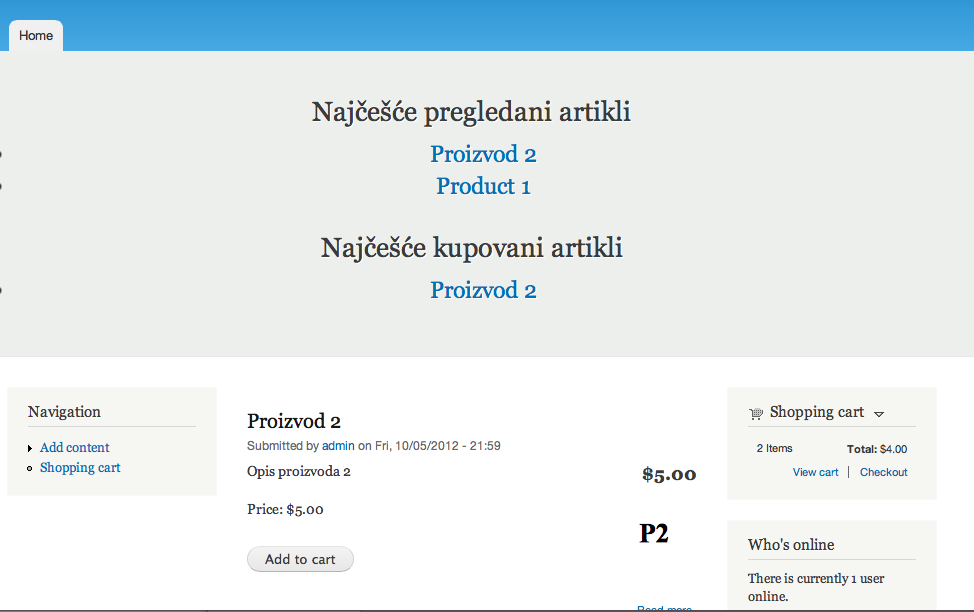
\includegraphics[width=10cm]{img/pregled_rezultata_preporuke.png}
\caption{Preporuka - informacije o najposjećivanijim i najviše kupovanim artiklima}
\end{figure}

\chapter {Sistem preporuke}
\vspace*{-0.7cm}

\section{Sistemi preporuke općenito}

Količina informacije koje internet korisnici dobijaju se stalno povećava. To za posljedicu ima sve teže i teže nalaženje relevatnih informacija. 
Zato su tehnike filterisanja relevatnih informacija dobile na velikoj važnosti. Set algoritama koji nastoje riješit taj problem nazivaju se
sistemi za kolaborativno filterisanje, odnosno sistemi preporuke (eng. CF - Collaborative Filtering recommender systems). 
CF algoritmi pohranjuju akcije koje pojedini korsinici vrše nad artiklima.
Ovi podaci se onda koriste da se generišu grupacije ("susjedstva") sličnih artikala ili korisnika sa pretpostavkom
da korisnik koji preferira iste stvari (proizvode, usluge) kao i korisnici koji su u bliskom susjedstvu sa njim\citep{bac_wien}

\section{Easyrec sistem preporuke}

Easyrec\footnote{\url{http://en.wikipedia.org/wiki/Easyrec}} je cjelovito rješenje sistema preporuke.

On kombinuje više algoritama za ragniranje artikala, te na osnovu njih davanje preporuke korisnicima sistema.

Easyrec ima sopstvenu bazu artikala prema kojoj vrši proračune. Ona prima podatke o akacijama korisnika nad pojedinim artiklima unutar e-commerce sistema, 
procesira ih putem algoritama preporuke, te korisnicima vraća rezultat u obliku rang-lista po više različitih kriterija.

Na njihovoj web stranici{\footnote\url{http://easyrec.org}} stoji:
\begin{quotation}
easyrec is:
\begin{itemize}
\item easy to use - personalize your application within minutes
\item easy to integrate - due to plugins, a REST API or placing javascript codesnippets in your web pages.
\item easy to scale - due to distributed architecture
\item easy to maintain - with the included management application
\item easyrec is OPEN SOURCE and FREE!
\end{itemize}
\end{quotation}

Može se reći da su većinu od ovih "easy" obećanja uspjeli postići.

\begin{figure}[H]
\centering
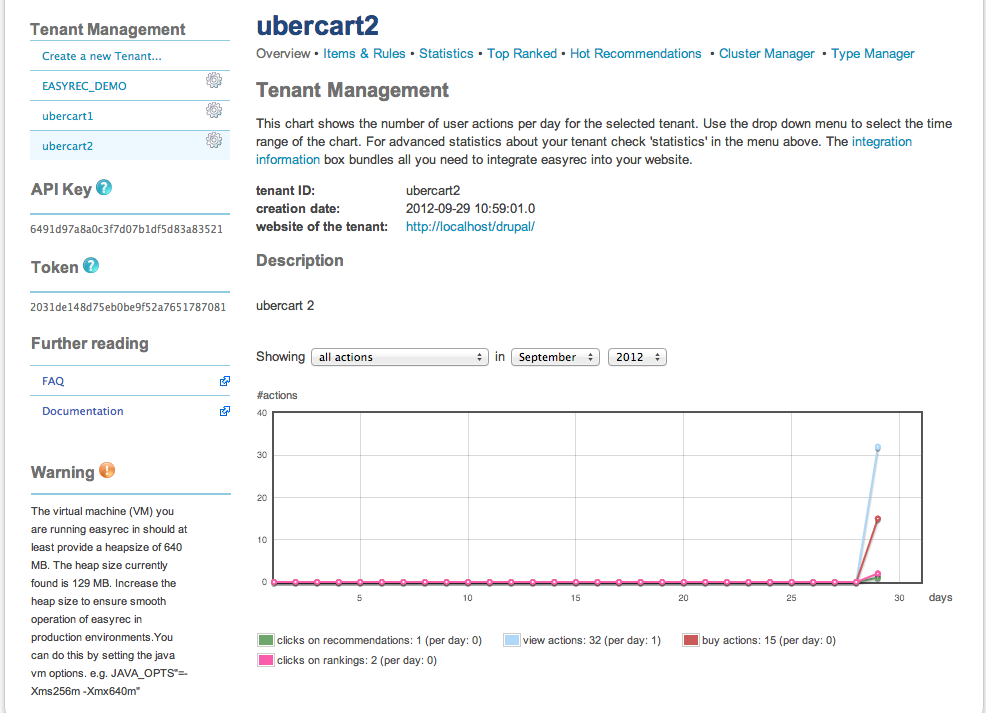
\includegraphics[width=12cm]{img/easyrec_1_tenant.png}
\caption{Easyrec "tenant" ubercart2}
\end{figure}

\begin{figure}[H]
\centering
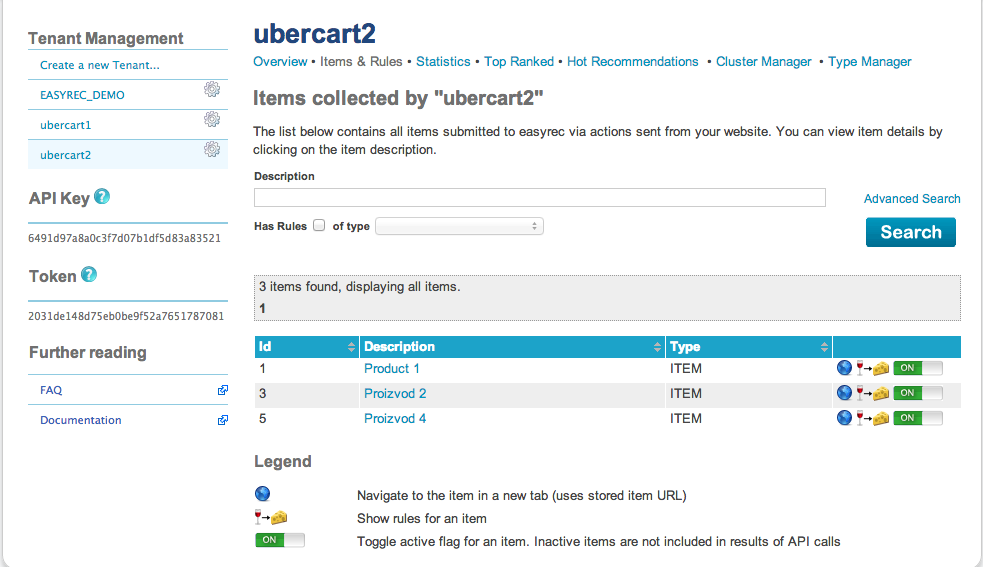
\includegraphics[width=12cm]{img/easyrec_2_item.png}
\caption{Easyrec "items" koje "tenant" ubercart2 bilježi}
\end{figure}


\begin{figure}[H]
\centering
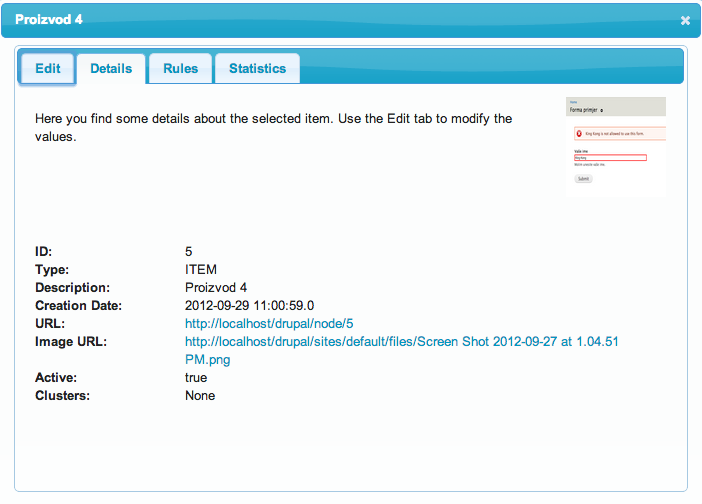
\includegraphics[width=12cm]{img/easyrec_3_item.png}
\caption{Easyrec prikaz jednog "item"-a}
\end{figure}

\begin{figure}[H]
\centering
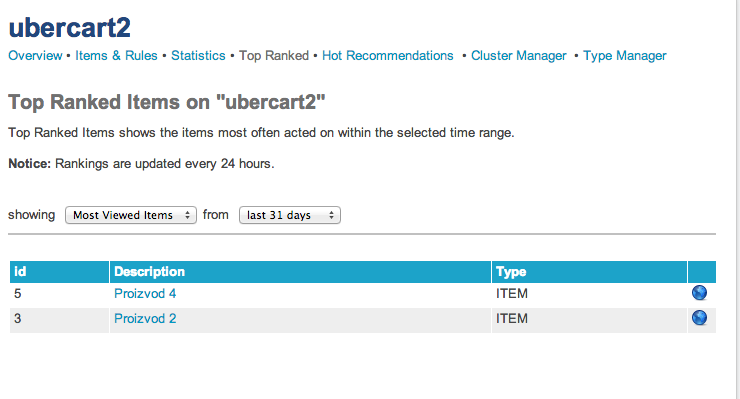
\includegraphics[width=12cm]{img/easyrec_4_top_ranked.png}
\caption{Easyrec "top ranked" artikli}
\end{figure}

\begin{figure}[H]
\centering
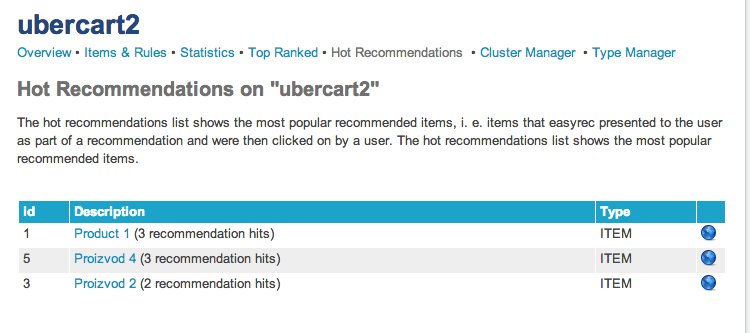
\includegraphics[width=12cm]{img/easyrec_5_hot_recommend.png}
\caption{Easyrec preporučeni ("hot recommend") artikli}
\end{figure}

\begin{figure}[H]
\centering
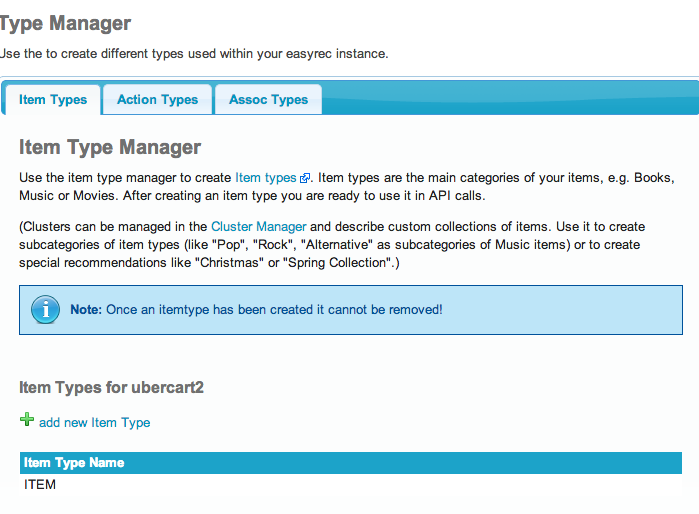
\includegraphics[width=12cm]{img/easyrec_6_item_types.png}
\caption{Easyrec tipovi "itema" (stavki koje ocjenjujemo i preporučujemo) }
\end{figure}

\begin{figure}[H]
\centering
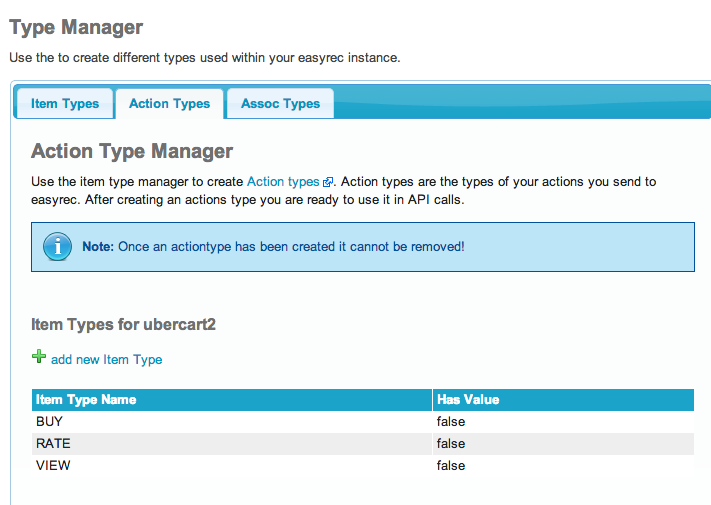
\includegraphics[width=12cm]{img/easyrec_7_item_actions.png}
\caption{Easyrec akcije koje se bilježe za stavke}
\end{figure}

\begin{figure}[H]
\centering
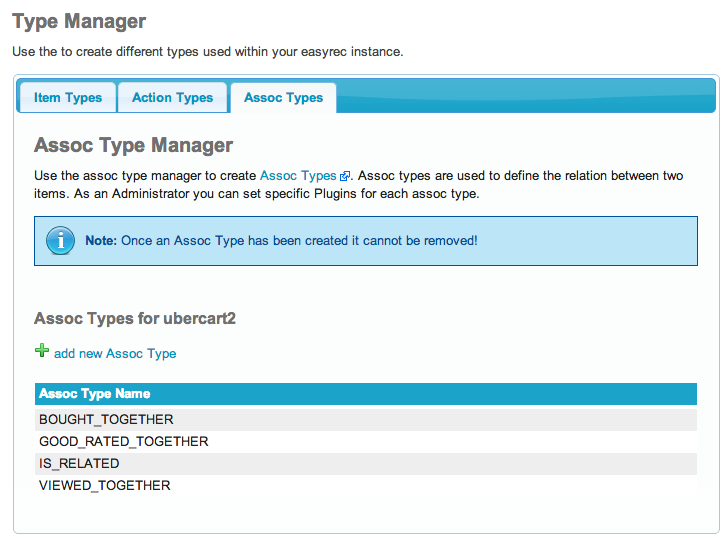
\includegraphics[width=12cm]{img/easyrec_8_item_assoc.png}
\caption{Easyrec asocijacije između stavki}
\end{figure}

\begin{figure}[H]
\centering
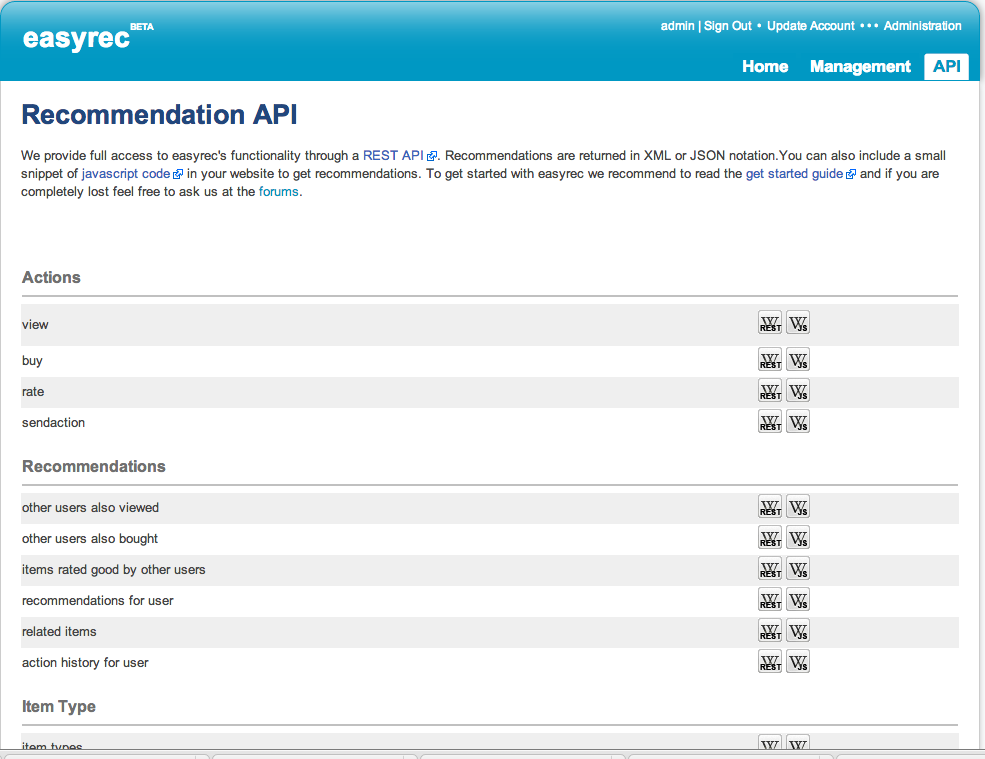
\includegraphics[width=12cm]{img/easyrec_9_recommend_api.png}
\caption{Easyrec API putem koje "third-party" e-commerce aplikacija pristupa}
\end{figure}

\begin{figure}[H]
\centering
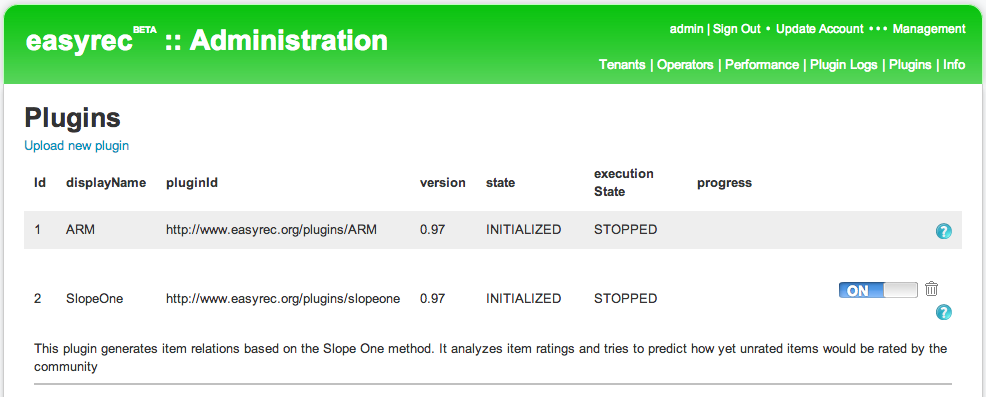
\includegraphics[width=12cm]{img/easyrec_10_plugins.png}
\caption{Algoritmi koji se primjenjuju su easyrec plugin-ovi}
\end{figure}


% -------------------------------------------------
\bibliography{literatura}
\bibliographystyle{fit}

% -------------------------------------------------
\appendix

\chapter{Software toolset}
\begin{enumerate}
  \item Mac OS X 10.8.2
  \item mvim, vim tekst editor ver 7.3
  \item MacTex (TeX Live 2012)
\end{enumerate}

\chapter{Software repozitoriji}

\begin{itemize}
  \item drupal web content framework \url{https://github.com/hernad/drupal}
  \item easyrec source code \url{https://github.com/hernad/easyrec}
  \item PeB izvorni kod seminarskog rada \url{https://github.com/hernad/FIT\_PeB}

\end{itemize}

\end{document}
